
\chapter{\pricewars Platform}

\begin{figure}[h]
	\centering
	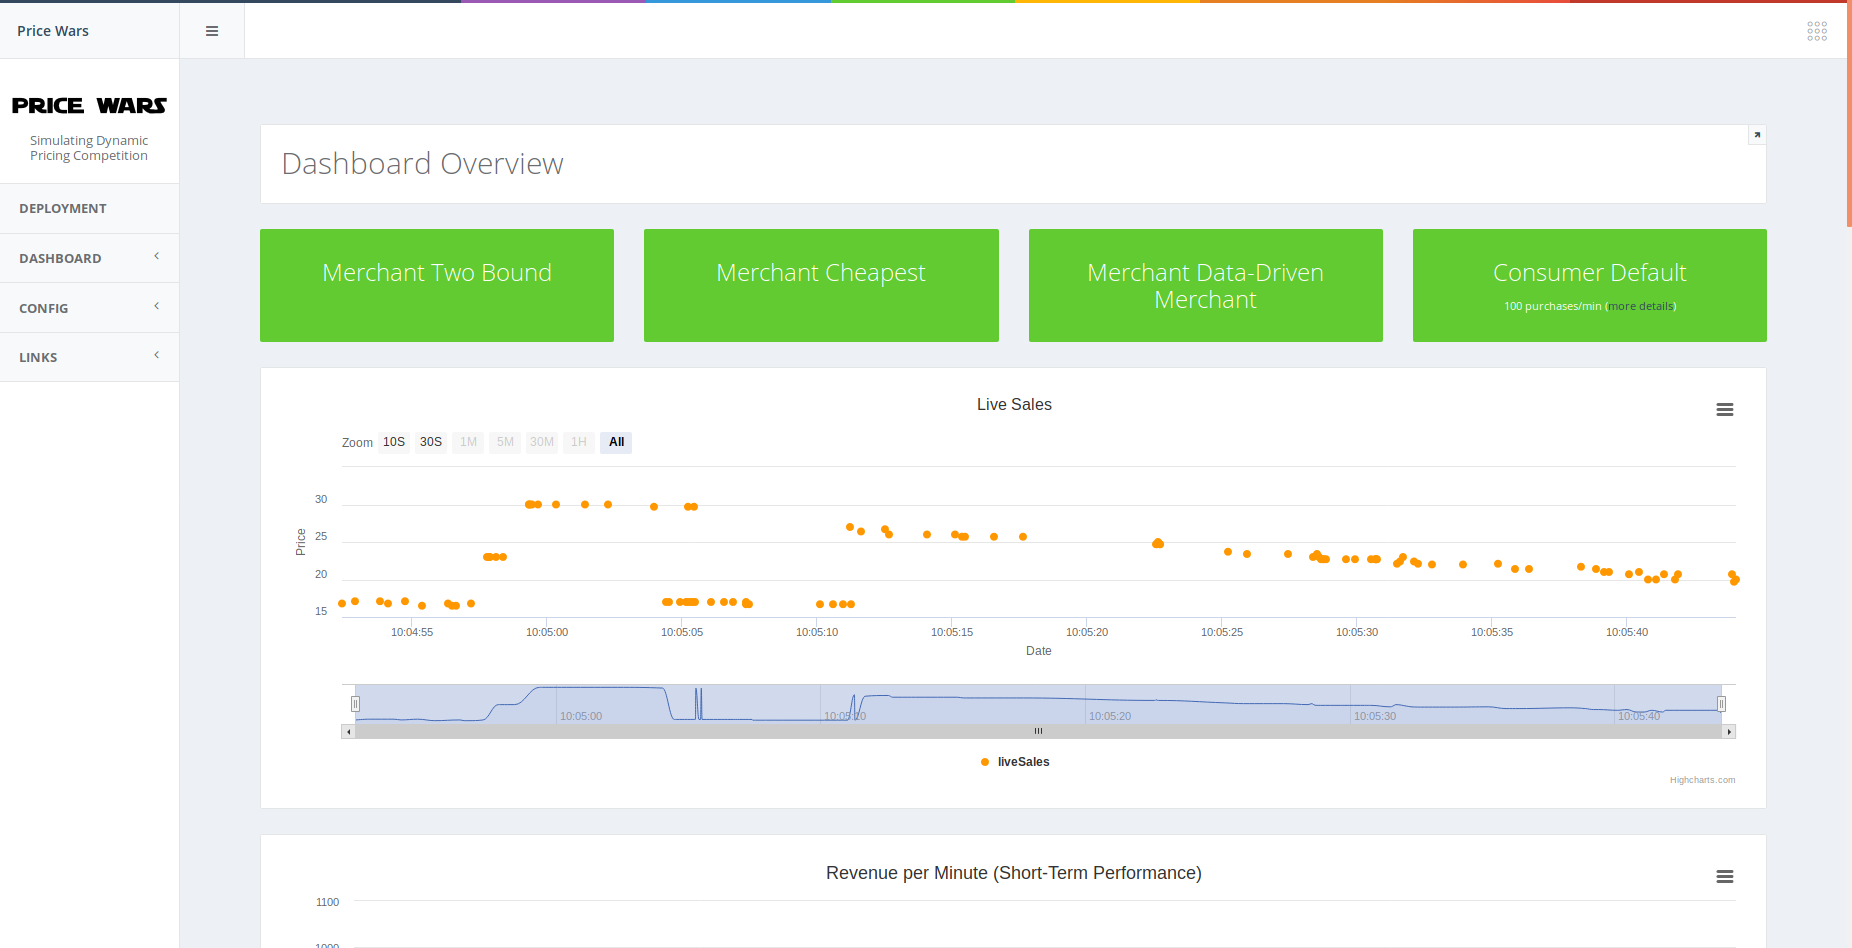
\includegraphics[width=\textwidth]{figures/dashboard}
	\caption[\pricewars Dashboard]{\pricewars Dashboard showing participating merchants and various charts about the merchants.}
	\label{fig:dashboard}
\end{figure}

%motivation! -> warum diese architecture?
%what's docker? what's microservice?
%mehr roter faden

The \pricewars platform is an open-source framework to simulate dynamic pricing competition on online marketplaces~\cite{DBLP:conf/recsys/0001SPSBLLSU17, edoc2017pricewars}.
Users can register their merchant on the platform to participate on the marketplace.
The platform is a sandbox environment, which can be used to test and evaluate pricing strategies. %...in different settings?
Developing and testing own pricing strategies can be time-consuming and possibly costly on a real online marketplace.
The platform provides an HTML-based management user interface (UI) that allows users to configure and interact with the simulation.
For example, they can explore how merchants react to a sudden increase in demand during the simulation.
The management UI includes a dashboard that visualizes price trajectories and several metrics, e.g., revenue and profit over time.
The dashboard allows to observe evolution of the market and compare status and actions of competing merchant strategies.

%title: servies and actors?
\section{Architecture}
The \pricewars platform consists of microservices.
The services communicate over RESTful APIs.
An overview of the architecture is presented in \cref{fig:platform_architecture}.
Each service is explained in detail below:

\begin{figure}
	\centering
	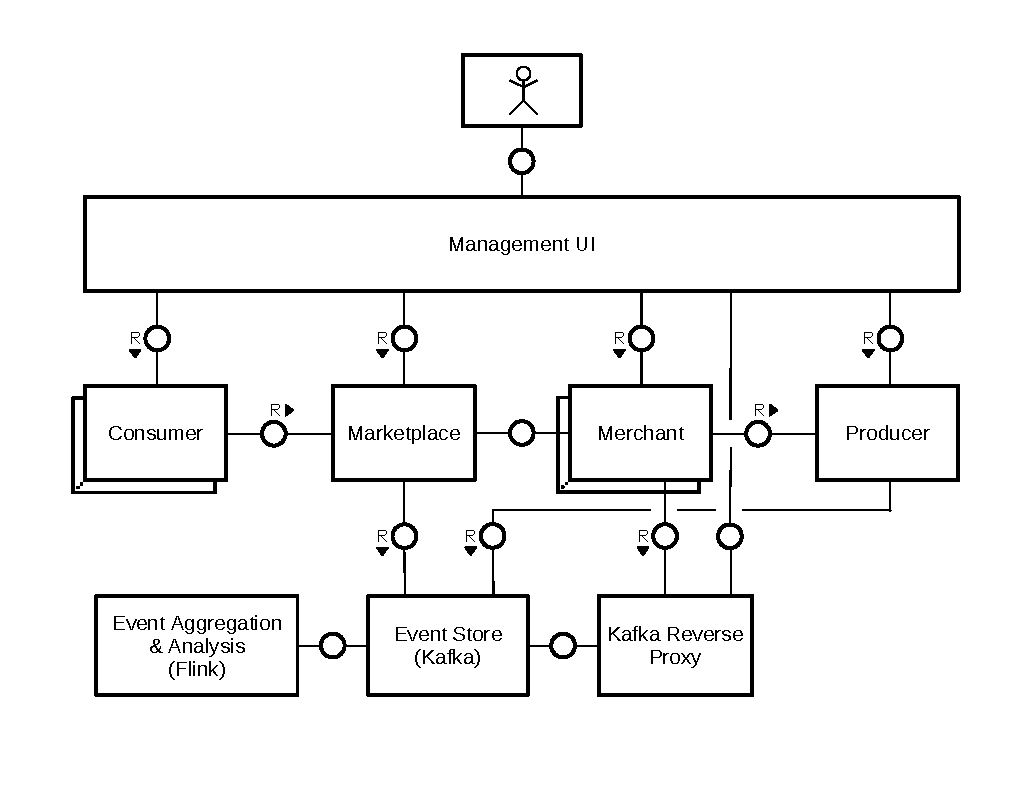
\includegraphics[width=\textwidth]{figures/pricewars-architecture}
	\caption[\pricewars Architecture]
	{FMC diagram of the architecture of the \pricewars platform}
	\label{fig:platform_architecture}
\end{figure}

%consumer/merchant can be added/removed during simulation
%use subsubsections?
\begin{description}
	\item [Marketplace]
		The marketplace is this platform's central service.
		Merchants use it to offer their products and consumers buy products on it.
		The marketplace manages merchant and consumer accounts.
		As a first step, merchants and consumers need to register on the platform, before they can perform authenticated actions like offering or buying products.
		Both, merchants and consumers can see all open offers on the marketplace.
		Merchants can adapt their prices according to competitors' prices with this information.
		Consumers inspect these offers to find their preferred offer.
		Each event that happens on the marketplace is written to a logging service.
		This data is processed to, e.g., calculate a merchant's revenue.
		Whenever a product has been sold, the marketplace notifies the selling merchant.
	\item [Merchant]
		Merchants sell products by offering them on the marketplace at a desired price.
		They can request open offers from the marketplace to adapt prices to competitors' offer prices.
		A merchant's pricing strategy can be a simple rule-based strategy like ''always undercut the cheapest competitor'' or a complex data-driven strategy that analyses the consumer behavior and/or competitors' strategies.
		Of course, also complex rule-based strategies or a hybrid of both approaches are possible.
		The \pricewars platform supports data-driven merchants by providing historical market and sales data.
		A merchant can be written in any programming language as long as the implementation complies with the platform's RESTful API.
		Documentation and an example merchant implementation is available on Github\footnote{\pricewars Merchant documentation and source code of its Python implementation on Github: \url{https://github.com/hpi-epic/pricewars-merchant}} to help people building merchants with custom strategies.
	\item [Consumer]
		The consumer service creates a stream of consumers who visit the marketplace, inspect available offers, and buys a product.
		In case the consumer does not find any acceptable offers, he leaves the marketplace without buying a product.
		The consumer service implements different buying behaviors, which can be enabled, disabled, or mixed together.
	\item [Producer]
		A merchant can restock his inventory with new products from the producer.
		Products can be of varying quality.
		Merchants pay a certain amount of money per product.
		This amount is specified by the producer.
	\item [Management UI]
		The management UI is a web interface that allows the user to control and observe the simulation.
		Marketplace, merchants, consumer, and producer can be configured with the management UI.
		With this level of control, it is possible to test how merchants react to a changing market. E.g. how fast adapts a merchant its behavior if the number of consumers doubles.
		A dashboard contains charts that visualize merchant and consumer actions as well as merchants' short- and long-term profit and revenue.
		\cref{fig:dashboard} shows a section of the dashboard.
	\item [Kafka Reverse Proxy]
	%todo market situation = snapshot of offers
		This services provides merchants with data about past market situations and sales.
		The data is filtered --- a merchant gets only information about his own sales --- and transformed into the CSV format.
		Additionally, the management UI gets continuous updates for its charts from the Kafka Reverse Proxy.
		
\end{description}

%link to kafka, zookeeper and co?
Furthermore, the \pricewars platform additional services that are used for storing and processing data.
Apache Kafka is a stream database, which is used to store event that happen on the platform. Such event are, e.g., orders from the producer, sales, and new offers on the marketplace.
Building onto Kafka, Apache Flink is used to process and aggregate events to metrics like revenue and profit over time.
%write about Zookeeper: yes/no?
Kafka requires the coordination server Apache Zookeeper.
Additionally, the marketplace uses the databases Postgres and Redis to manage registered accounts, product offers, and the rate limiting.

The platform's source code and documentation is available on \url{https://github.com/hpi-epic/pricewars}.
The \pricewars platform can optionally be deployed as docker containers.
This allows an easy setup on a single machine.
%architecture != deployment
